\section{(5,5) Carbon Nanotube --- Transport properites}
\label{sec13:cnt}

\begin{itemize}
\item Outline: {\it Obtain the bandstructure, quantum conductance and density of states of a metallic (5,5)
carbon nanotube.}
\end{itemize}

\begin{figure}[h!]
\centering
\subfloat[side view]{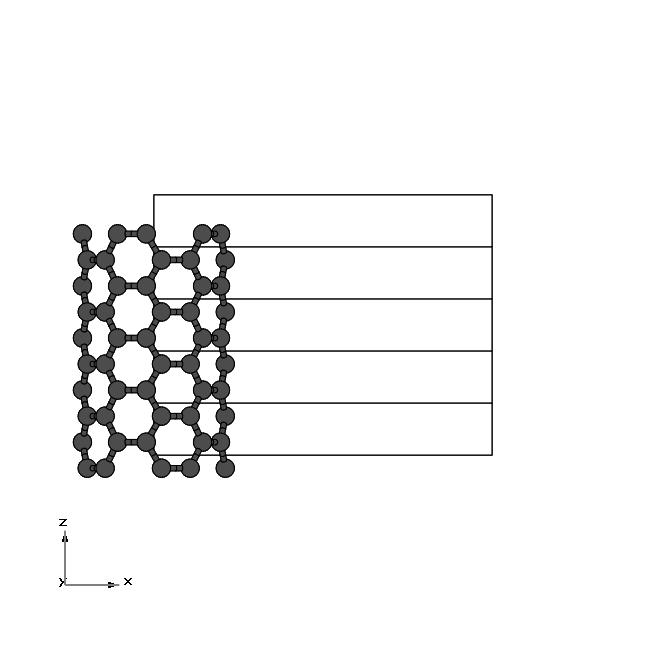
\includegraphics[width=0.25\columnwidth,trim={45pt 55pt 45pt 55pt},clip]{figure/example13/cnt55_1.png}}
\centering
\subfloat[prospectic top view]{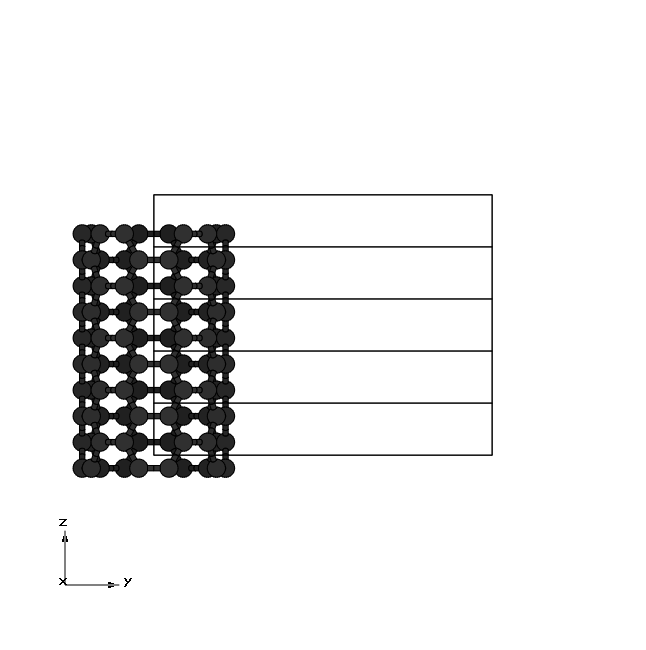
\includegraphics[width=0.25\columnwidth,trim={45pt 45pt 45pt 55pt},clip]{figure/example13/cnt55_2.png}}
\caption{5 unit cells for the carbon nanotube system from a) side view and b) prospective top view plotted with the \xcrysden{} program.}
\label{fig13.0}
\end{figure}

\begin{itemize}
\item[1] {\it Run pwscf and {\tt wannier90}. Inspect the output file {\tt cnt55.wout}. The minimisation of the spread occurs in a two-step proce-
dure. First, we minimise $\Omega_I$. Then, we minimise $\Omega_D + \Omega_{OD}$.}

Below, an extract from the {\tt .wout} file showing a summary of the disentanglement procedure (minimisation of $\Omega_I$)
\end{itemize}
\begin{tcolorbox}[floatplacement=h!,float,nobeforeafter,sharp corners,boxrule=0.5pt]
\small{
	\begin{verbatim}
                   Extraction of optimally-connected subspace                  
                   ------------------------------------------                  
 +---------------------------------------------------------------------+<-- DIS
 |  Iter     Omega_I(i-1)      Omega_I(i)      Delta (frac.)    Time   |<-- DIS
 +---------------------------------------------------------------------+<-- DIS
       1      33.96797815      33.91073784       1.688E-03      0.00    <-- DIS
       2      33.92937273      33.90274574       7.854E-04      0.02    <-- DIS
       .		.					.				.			 .
       .		.					.				.			 .

      45      33.89889125      33.89889125       4.172E-11      0.50    <-- DIS
      46      33.89889125      33.89889125       1.626E-11      0.51    <-- DIS

             <<<      Delta < 1.000E-10  over  3 iterations     >>>
             <<< Disentanglement convergence criteria satisfied >>>

        Final Omega_I    33.89889125 (Ang^2)

 +----------------------------------------------------------------------------+
	\end{verbatim}
}
\end{tcolorbox}

\newpage
Below, an extract from the {\tt .wout} file showing the final state for the minimisation of $\Omega_D + \Omega_{OD}s$
\begin{tcolorbox}[sharp corners,boxrule=0.5pt]
\small{
\begin{verbatim}
    	 Final State
  WF centre and spread    1  ( -6.875141,  7.935472,  7.937658 )     0.65233309
  WF centre and spread    2  (  4.748245,  7.935472,  7.937658 )     0.65234300
  WF centre and spread    3  (  5.809324,  6.097678,  7.937658 )     0.65186298
  WF centre and spread    4  (  7.816785, -7.396927,  7.648002 )     1.20135958
  WF centre and spread    5  (  7.816785, -7.396927, -7.648002 )     1.20135948
  WF centre and spread    6  (  7.936083,  7.324218, -7.937658 )     0.60992987
  WF centre and spread    7  (  7.935073, -6.095184,  7.937658 )     0.65161009
  WF centre and spread    8  (  6.874208, -6.712573,  7.937658 )     0.61134798
  WF centre and spread    9  (  6.874224,  6.850489, -7.648754 )     1.20500764
  WF centre and spread   10  ( -7.936214,  6.097679,  7.937658 )     0.65186256
  WF centre and spread   11  (  5.813353, -6.095183,  7.937658 )     0.65160955
  WF centre and spread   12  (  6.874224,  6.850489,  7.648754 )     1.20500766
  WF centre and spread   13  (  5.812342,  7.324217,  7.937658 )     0.60993084
  WF centre and spread   14  (  5.931632, -7.396946,  7.648001 )     1.20136423
  WF centre and spread   15  (  5.931632, -7.396946, -7.648001 )     1.20136424
  Sum of centres and spreads ( 71.362557,  7.925029, 55.563607 )    12.95829277
 
         Spreads (Ang^2)       Omega I      =    10.455434168
        ================       Omega D      =     0.000000000
                               Omega OD     =     2.502858604
    Final Spread (Ang^2)       Omega Total  =    12.958292772
 ------------------------------------------------------------------------------
 \end{verbatim}
 }
 \end{tcolorbox}


\begin{enumerate}\addtocounter{enumi}{1}
 \item {\it Note that the initial $p_z$ projections on the carbon atoms are oriented in the radial direction with
respect to the nanotube axis.}

{\tt
\begin{quote}

Begin Projections

Ang

c=   3.3780, -0.7128, -0.6157 :pz {\color{red}:z=  3.3780, -0.7128,  0.0000 :x=0,0,1}

\end{quote}
}

\item {\it The interpolated bandstructure is written to {\tt cnt55\_band.agr}}

To plot the interpolated bands, the quantum conductance and the Density of States as shown in Fig. 6 in the {\sc Wannier90} tutorial, one can use the {\tt xmgrace} program.
\end{enumerate}

\begin{tcolorbox}[colback=blue!5!white,title=XMGRACE TUTORIAL] 
Run the {\tt xmgrace} plotting program from command line as 

{\tt 
\begin{quote}
\$ > xmgrace
\end{quote}
}

Before importing the data to be plotted, we have to reorganize the layout by selecting

{\tt

\begin{quote}

Edit $\mapsto$ Arrange graphs\dots

\end{quote}
}
here we can generate a grid of graphs by selecting the number of columns and rows from the drop menus. For this particular example, we want to increase the number of columns to 3, i.e. {\tt Cols: 3} and leave the number of rows to 1 in the {\tt Matrix} section. Moreover, we don't want any gap between the graphs so we also need to modify the value of {\tt Hgap/width} in the bottom {\tt Spacing} section, i.e {\tt Hgap/width 0}. Once we have generated the three graphs we need to import the data. This can be achieved by 
{\tt \begin{quote}
Data $\mapsto$ Import $\mapsto$ ASCII\dots
\end{quote}}

The three files to import are {\tt cnt\_band.agr}, {\tt cnt\_qc.dat} and {\tt cnt\_dos.dat}, respectively. For each file we need to select the graph in the {\tt Read to graph:} section, i.e. {\tt G(0), G(1)} and {\tt G(2)}, respectively.

In order to flip the x-axis with the y-axis, one need to perform the following
{\tt
\begin{quote}
Data $\mapsto$ Transformations $\mapsto$ Evaluate expressions\dots
\end{quote}	
}
In the {\tt Formula:} section write
{\tt
\begin{quote}
s1.x=s0.y; s1.y=s0.x
\end{quote}}
and then click {\tt apply}.
\end{tcolorbox}



\begin{figure}[b!]
\centering
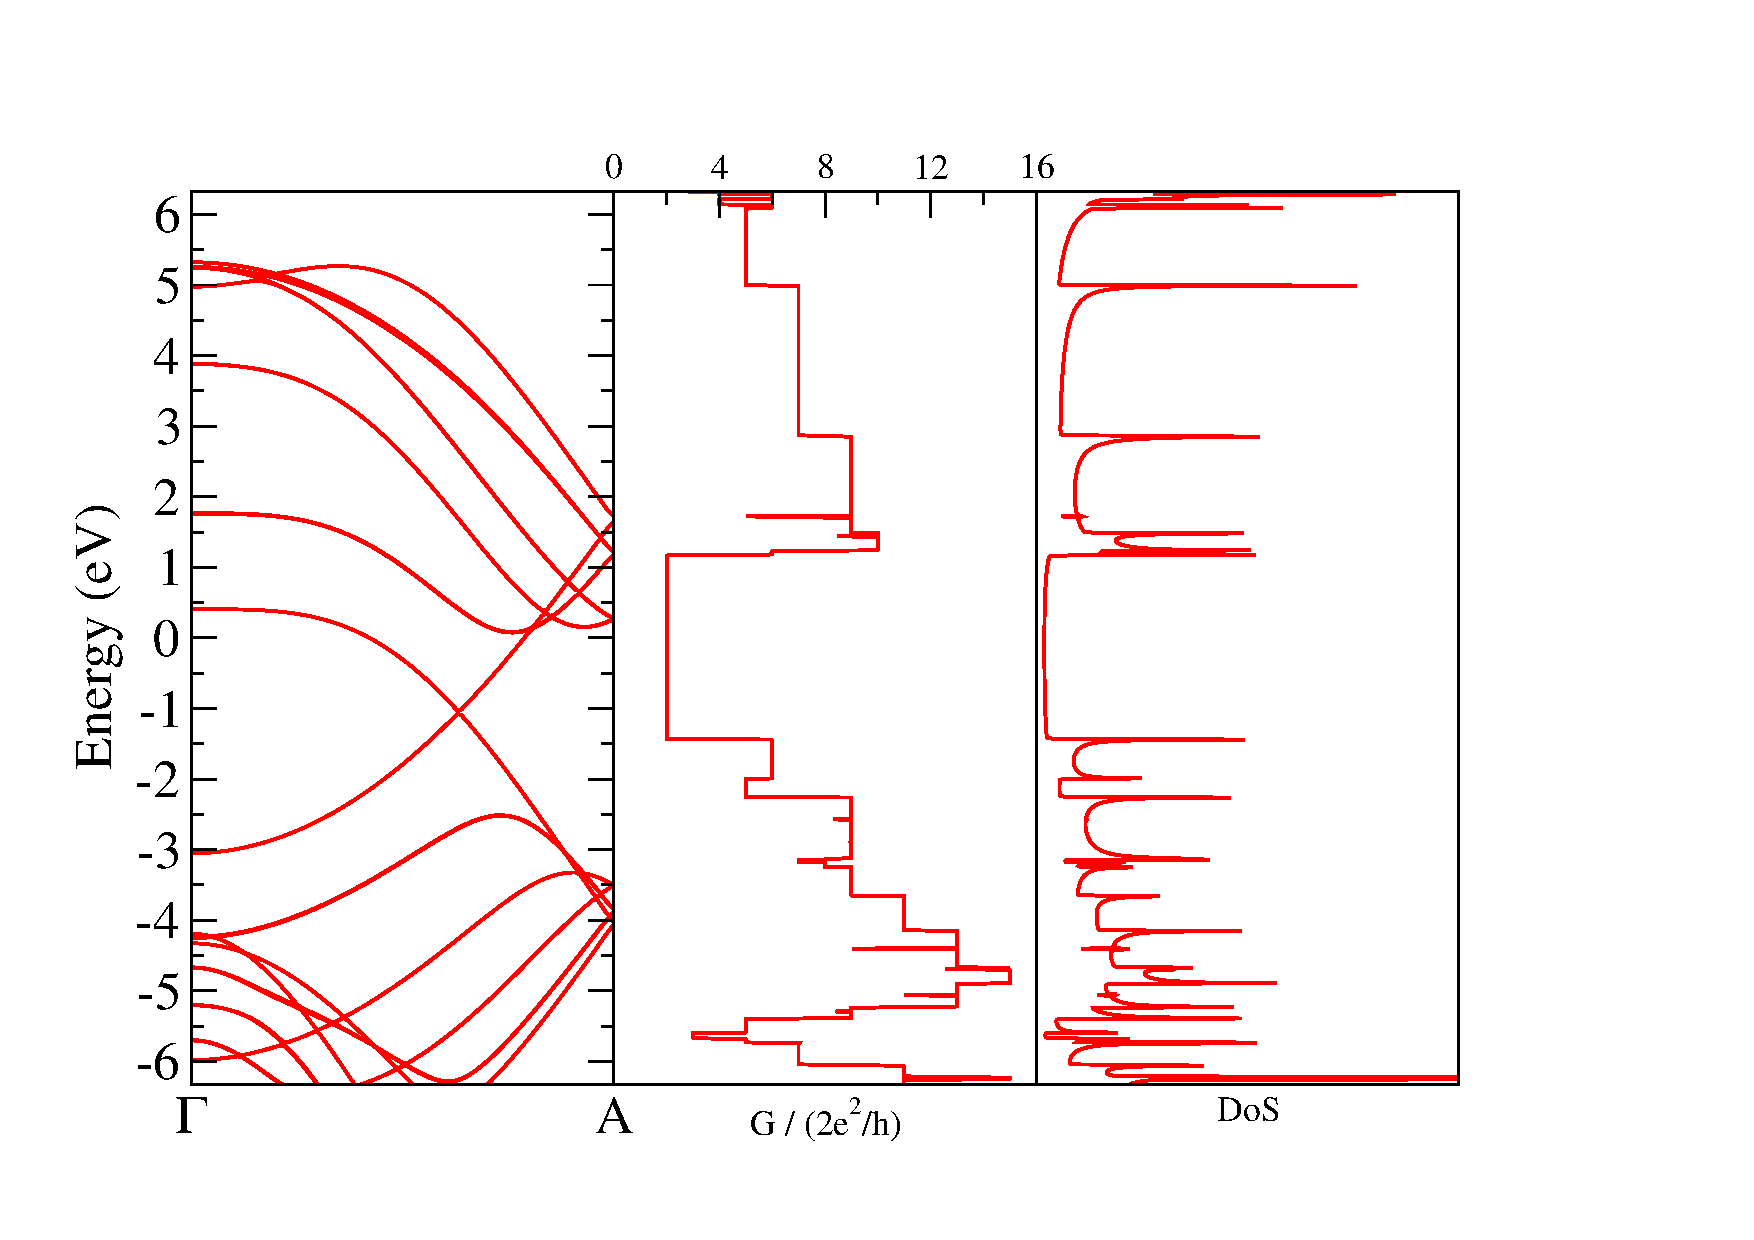
\includegraphics[width=0.7\columnwidth]{figure/example13/cnt55_band.pdf}
\caption{Reproduction of Fig. 6 in the {\sc wannier90} tutorial.}\label{fig13.1}
\end{figure}
